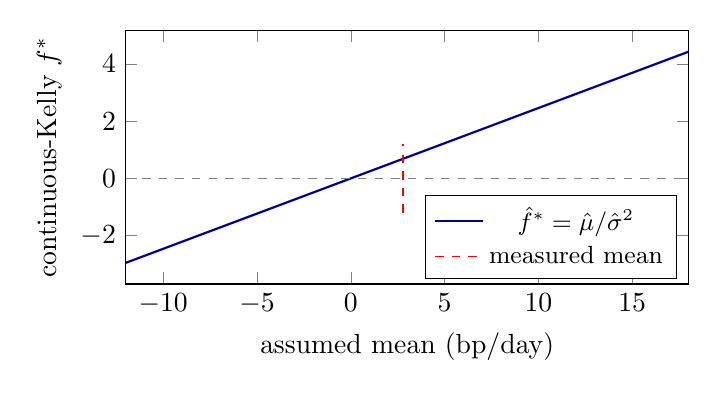
\begin{tikzpicture}
\begin{axis}[width=0.72\linewidth, height=4.8cm, xlabel={assumed mean (bp/day)},
  ylabel={continuous-Kelly $f^*$}, xmin=-12, xmax=18,
  legend style={at={(0.98,0.02)},anchor=south east,font=\small}]
\addplot[blue!60!black, thick, domain=-12:18, samples=60] {x*1e-4/4.07e-4};
\addplot[red, dashed] coordinates {(2.78,-1.2) (2.78,1.2)};
\addplot[gray, dashed, domain=-12:18] {0};
\legend{$\hat f^*=\hat\mu/\hat\sigma^2$, measured mean}
\end{axis}
\end{tikzpicture}
